\chapter{Approach}
\label{ch:approach}

\section{Overview}

\noindent
    
    This thesis addresses the problem of multimodal fact verification, where a claim consists of both textual and visual content, and the objective is to retrieve relevant evidence for verification. Compared to traditional text-only fact-checking, multimodal verification introduces additional complexity due to the need to analyze cross-modal relationships between the claim text and associated image.


The proposed system decomposes multimodal fact verification into a sequence of retrieval and reasoning stages. To investigate the impact of retrieval and question-generation strategies, two alternative pipelines are explored.

The first approach follows an \textit{iterative question-answer generation} strategy. The Vision-Language Model (VLM) generates a verification question, retrieves evidence from the multimodal knowledge store, answers the question, and then uses the accumulated evidence to generate subsequent questions. This process continues until pre-defined number of iterations.

The second approach follows \textit{Claim Based Retrieval for QA generation (single pass)} strategy. Relevant evidence is retrieved directly from the claim using the proposed \textit{Dual-RAG} retrieval pipeline. The retrieved evidence is then provided to the VLM, which generates multiple question-answer pairs in a single pass before predicting the final verdict and justification.

Both approaches utilize the same multimodal retrieval infrastructure consisting of SPLADE, BGE, and LongCLIP retrieval, followed by Reciprocal Rank Fusion (RRF), cross-encoder reranking, and Maximal Marginal Relevance (MMR) diversification. The generated question-answer pairs and supporting evidence are subsequently used by the VLM to produce a verdict and evidence-grounded justification.


\section{Fact checking Pipeline Overview}

There are some important keywords that will be used throughout this section which were described in ~\citet{Cao2025May}.
\begin{itemize}
\item Claim Text: The text that needs to be fact checked
\item Claim Image: The image that comes along with the claim text that needs to be fact checked
    \item Question: The generated essential questions for verifying the image-text claim.
    \item Evidence: The retrieved textual and image information from the knowledge store based on the claim text, claim image and question
    \item Answer: The answer to the question based on the evidences retrieved
    \item Verdict: The predicted veracity label of the claim
    \item Justification: A textual justification that explains how a verdict can be reached on the basis of the evidence found
\end{itemize}

This thesis adopts the Team Factiverse system as its baseline architecture. The original system employs iterative question generation with modality-aware retrieval, where text-related questions are answered through SPLADE-based retrieval and image-related questions through CLIP-based retrieval. Retrieved evidence is subsequently aggregated and provided to the verification and justification modules. Building upon this architecture, this work investigates alternative retrieval strategies, evidence fusion mechanisms, and question-answer generation approaches, including both iterative and single pass paradigms, to improve multimodal fact verification performance.

\begin{figure}[ht]
\centering
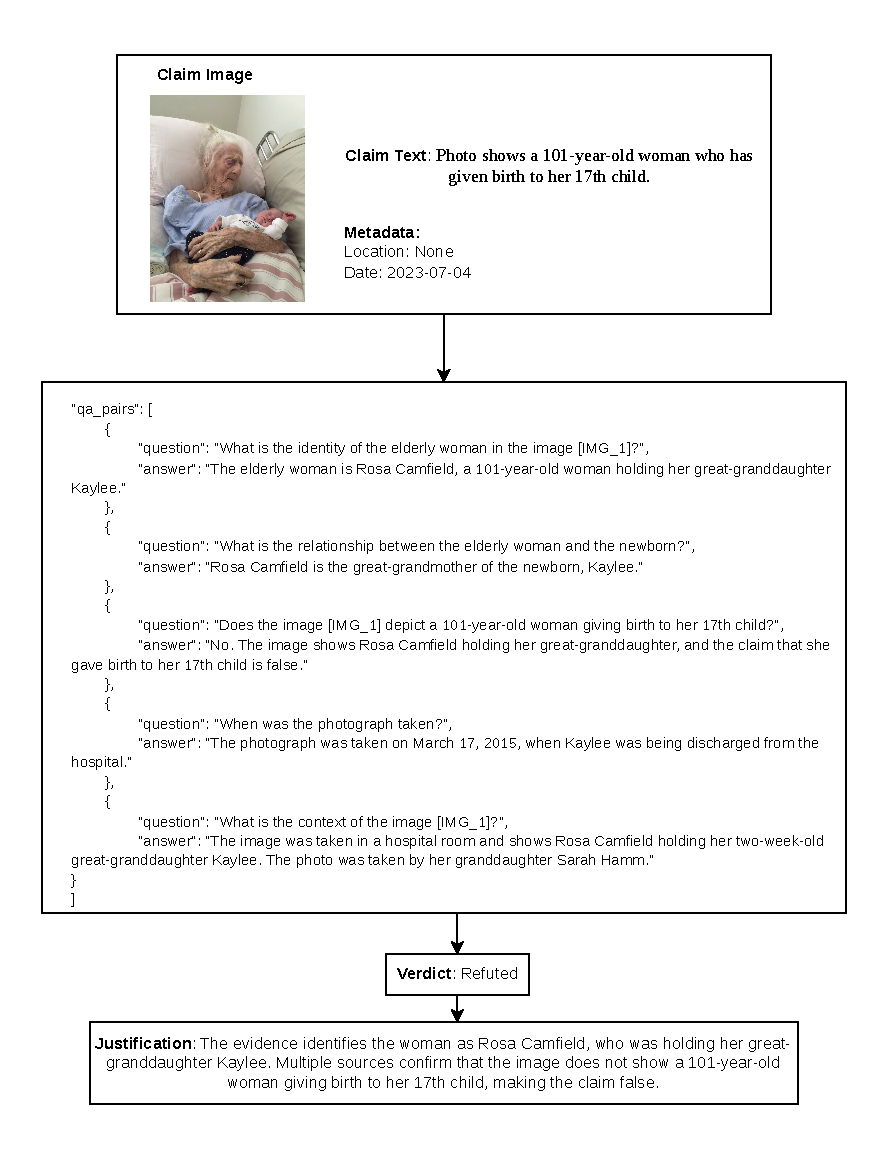
\includegraphics[width=\textwidth]{images/example1.pdf}
\caption{Overview of the different stages of the pipeline with an example}
\label{fig:example1}
\end{figure}

\vspace{2cm}

\section{Information Retrieval Strategies}

Evidence retrieval is a fundamental component of multimodal fact-checking. Given a textual claim and an associated image, the objective is to retrieve relevant evidence from a multimodal knowledge store that can support or refute the claim. Compared to traditional text-only fact-checking, multimodal verification introduces several additional challenges:

\begin{itemize}
\item \textbf{Long and noisy evidence sources}: Real-world evidence ranges from short snippets to lengthy news articles, making efficient retrieval difficult.

\item \textbf{Entity ambiguity and identity mismatch}: The same image may appear in multiple contexts and be associated with conflicting narratives, requiring careful disambiguation across sources.

\item \textbf{Image reuse and miscontextualization}: Images are frequently reused in unrelated contexts, creating misleading associations that cannot be detected through textual retrieval alone.

\item \textbf{Heterogeneous information signals}: Relevant evidence may be distributed across textual content, visual content, and metadata, requiring retrieval across multiple modalities.

\end{itemize}

To address these challenges, this thesis proposes a hybrid multimodal dual-branch retrieval architecture. The text retrieval branch combines sparse lexical retrieval (SPLADE) and dense semantic retrieval (BGE), while the image retrieval branch utilizes LongCLIP to retrieve image-related textual and visual evidence through image-text and image-image alignment.

\subsection{Sparse Lexical Retrieval using Splade}
The system employs SPLADE (Sparse Lexical and Expansion Model), a sparse neural retrieval model that combines exact lexical matching with learned term expansion. Unlike BM25, SPLADE can retrieve evidence containing semantically related terms and paraphrases that do not exactly match the query, helping to reduce vocabulary mismatch while preserving the efficiency and interpretability of sparse retrieval ~\cite{Formal2021Sep}.

Fact-checking frequently relies on exact matching of entities, dates, locations, numerical values, and quoted statements. Although dense retrieval is effective for semantic matching, it may fail to prioritize evidence containing these critical factual details. SPLADE addresses this limitation by preserving lexical signals while expanding queries and documents with semantically related terms.

SPLADE represents a query or document as a sparse vector over the BERT WordPiece vocabulary $\mathcal{V}$. Given an input sequence $x=(x_1,\ldots,x_n)$, token-level vocabulary activations are first computed using the masked language modeling (MLM) head. These activations are then transformed using ReLU and logarithmic saturation and aggregated across all token positions to obtain the final sparse representation:

\begin{equation}
s_j(x)=\sum_{i=1}^{n}\log\!\big(1+\operatorname{ReLU}(w_{ij})\big),
\quad j\in\mathcal{V}
\label{eq:splade_representation}
\end{equation}

where $w_{ij}$ denotes the activation score of vocabulary term $j$ at token position $i$.

The relevance between a query $q$ and a document $d$ is computed using a sparse dot product:

\begin{equation}
\operatorname{score}(q,d)
=
\langle s(q).s(d)\rangle
\label{eq:splade_score}
\end{equation}

The resulting SPLADE scores are used to rank documents, and the top 50 candidates are forwarded to the Reciprocal Rank Fusion stage for combination with dense retrieval results.

\subsection{Dense Semantic Retrieval using BGE(BAAI General Embedding)}

Dense retrieval represents text as continuous vector embeddings, enabling semantic matching beyond exact keyword overlap. This work employs BGE (BAAI General Embedding), specifically the \texttt{BAAI/bge-large-en-v1.5} model, as the primary dense retriever. BGE-large-en-v1.5 is a sentence transformer that produces 1024-dimensional embeddings and encodes queries and documents into a shared semantic space, allowing semantically related evidence to be retrieved even when the wording differs substantially from the claim.

The BAAI/bge-large-en-v1.5 model was selected because it provides high-quality semantic embeddings for English retrieval tasks and has demonstrated strong performance across a wide range of retrieval benchmarks . While alternative models such as mxbai-embed-large-v1 were considered, BGE was chosen due to its widespread adoption in retrieval-augmented generation systems, strong retrieval effectiveness, and straightforward integration with the FAISS-based indexing pipeline used in this work.

Although SPLADE incorporates learned term expansion, it remains a sparse retrieval model that relies on matching activated vocabulary terms. As a result, SPLADE excels at retrieving evidence containing exact entities, dates, locations, and numerical information. However, relevant evidence may sometimes be expressed using substantially different vocabulary or paraphrased descriptions.

To address this limitation, BGE is employed as a complementary dense retriever. By mapping queries and documents into a continuous semantic embedding space, BGE enables retrieval based on overall semantic similarity rather than vocabulary overlap. Combining BGE and SPLADE therefore allows the retrieval pipeline to benefit from both lexical precision and semantic generalization, improving evidence coverage for fact-checking claims.

Given a query embedding $\mathbf{q}$ and a document embedding $\mathbf{d}$, semantic relevance is computed using cosine similarity:
\begin{equation}
\label{eq:bge_cosine_similarity}
    \text{cos\_sim}(\mathbf{e}_i, \mathbf{e}_j) = \frac{\mathbf{e}_i \cdot \mathbf{e}_j}{\|\mathbf{e}_i\| \cdot \|\mathbf{e}_j\|} = \mathbf{e}_i \cdot \mathbf{e}_j \quad \text{(when } \|\mathbf{e}_i\| = \|\mathbf{e}_j\| = 1\text{)}
\end{equation}

where $\mathbf{e}_i$ and $\mathbf{e}_j$ denote the normalized embedding vectors of the query and document, respectively, $\mathbf{e}_i \cdot \mathbf{e}_j$ represents their dot product, and $\|\cdot\|$ denotes the Euclidean norm. Since BGE embeddings are L2-normalized before indexing and retrieval, cosine similarity is equivalent to the dot product between the embeddings.


Documents are ranked according to their cosine similarity scores, and the top 50 retrieved documents are forwarded to the Reciprocal Rank Fusion (RRF) stage for combination with the SPLADE retrieval results.




\subsection{Multomodal Retrieval using LongCLIP}

Textual retrieval alone is insufficient for multimodal misinformation because images are frequently reused in unrelated or misleading contexts. To address this issue, this work incorporates LongCLIP for image-based retrieval.

LongCLIP was selected as the visual retrieval model because the retrieval task in this work involves matching claim images against image-related textual descriptions and evidence passages contained within the multimodal knowledge store. Unlike the original CLIP architecture, LongCLIP extends the text context length from 77 to 248 tokens, enabling longer image descriptions and evidence passages to be encoded without severe truncation ~\cite{Zhang2024Mar}. This characteristic is particularly relevant for multimodal fact-checking, where image-related evidence often consists of detailed descriptions and news passages rather than short captions.

Alternative models such as SigLIP and ColPali were considered during system design. However, SigLIP is primarily optimized for image-text alignment with relatively short textual inputs ~\cite{Zhai2023Mar}, while ColPali is designed for visual document retrieval, where entire document pages are represented and retrieved as images ~\cite{Faysse2024Jun}. In contrast, the knowledge store used in this work consists of textual evidence passages, image-related textual descriptions, and image embeddings rather than scanned document pages. Consequently, LongCLIP was selected because its retrieval formulation aligns naturally with the structure of the proposed knowledge store and supports the longer textual contexts commonly encountered in multimodal fact-checking.

For these reasons, LongCLIP was adopted as the visual retrieval component of the proposed Dual-RAG retrieval pipeline.

LongCLIP retrieves the top 50 documents based on the claim image, captions and questions and provides them to the next stage along with top 3 images.


\section{Indexing the Knowledge Store}

The knowledge store in AVerImaTeC contains documents of highly variable length, ranging from short social media posts of a few dozen words to full-length news articles exceeding tens of thousands of words. Encoding entire documents as single vectors leads to information dilution, where the embedding averages over large spans of text and loses the fine-grained details needed for fact verification. Conversely, encoding at the sentence level produces fragments that lack sufficient context to be meaningfully matched against a claim. To address this, each retrieval system adopts a chunking strategy tailored to its encoding model before building its respective index.

\begin{figure}[ht]
\centering
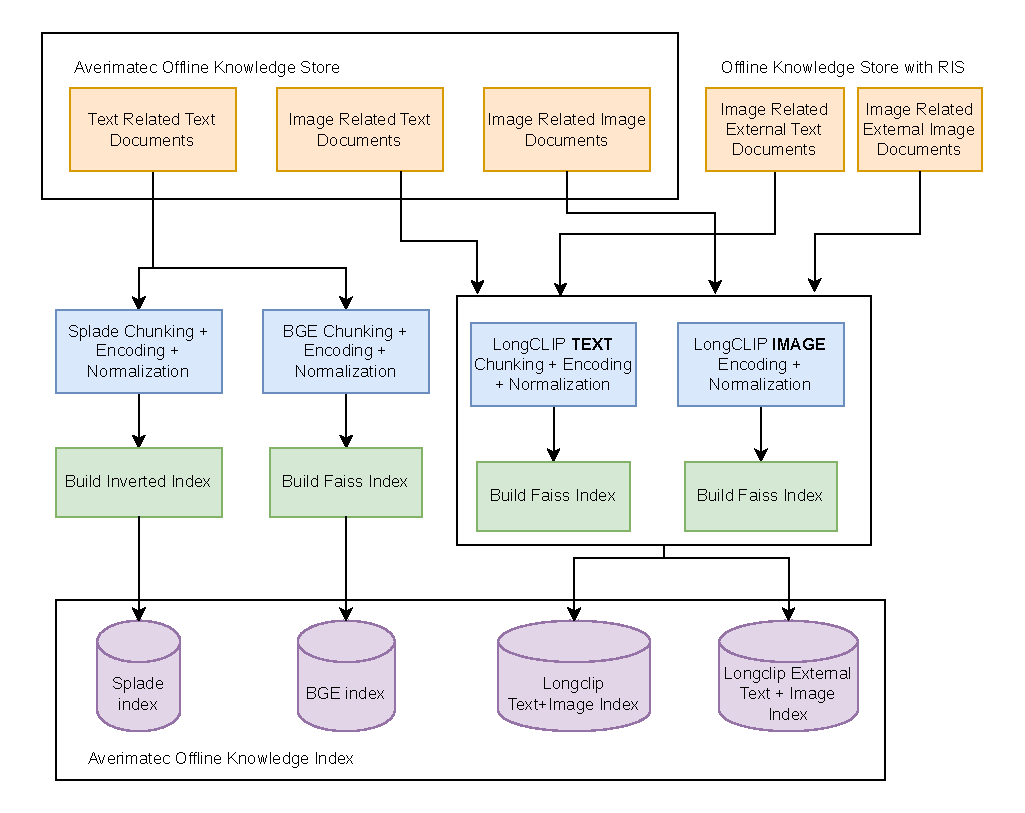
\includegraphics[width=\textwidth]{images/KnowledgeStore.pdf}
\caption{Knowledge Store Setup with different embeddings from different sources. The orange sections are the different sources of documents, blue sections are related to chunking, encoding and normalization, green sections are for building the index and the purple sections are the final indexes for specific retrieval methods}
\label{fig:knowledgestore}
\end{figure}

The three retrieval systems — BGE, SPLADE, and LongCLIP — differ in their chunking granularity, encoding methodology, and index structure. An overview of the process used to index the knowledge store using these three retrieval systems is shown in Fig~\ref{fig:knowledgestore}. Table~\ref{tab:chunking_comparison} summarizes the differences.

\begin{table}[htbp]
\centering
\caption{Comparison of chunking, encoding, and indexing across the three retrieval systems.}
\label{tab:chunking_comparison}
\begin{tabular}{lccc}
\hline
\textbf{Aspect} & \textbf{BGE} & \textbf{SPLADE} & \textbf{LongCLIP} \\
\hline
Chunk size (words) & 256 & 200 & 248 \\
Overlap (words) & 50 & 0 & 50 \\
Embedding type & Dense (1024-d) & Sparse (vocab-sized) & Dense (768-d) \\
Index structure & FAISS & Inverted index & FAISS \\
Modality & Text & Text & Text + Images \\
Similarity metric & Cosine (via IP) & Dot product & Cosine (via IP) \\
\hline
\end{tabular}
\end{table}

\subsection{Chunking Strategies}

All three retrieval systems segment documents into smaller chunks before encoding, but each uses different chunk sizes and overlap settings optimized for its respective model.

\subsubsection{BGE Chunking}

Documents are split into fixed-size chunks of 256 words with an overlap of 50 words between consecutive chunks. The larger chunk size enables the dense encoder to capture broader contextual relationships, while the overlap ensures that relevant information near chunk boundaries is preserved. Documents shorter than 256 words are treated as a single chunk.


Fixed-size chunking was selected instead of semantic chunking. Although semantic chunking, which partitions documents into semantically coherent segments, has gained popularity in Retrieval-Augmented Generation (RAG) systems, recent studies suggest that its benefits are often outweighed by the additional computational overhead ~\cite{Qu2024Oct}. Furthermore, retrieval performance is frequently influenced more by embedding quality than by the chunking strategy itself. Given that the knowledge store consists of real-world news articles and web documents, fixed-size chunking with overlap was adopted as a robust and computationally efficient preprocessing strategy.


For a document represented as a sequence of words $w_1,w_2,\ldots,w_n$, the $i$-th chunk is defined as

\begin{equation}
c_i =
(w_{s_i}, w_{s_i+1}, \ldots, w_{s_i+L-1}),
\qquad
s_i = i(L-O)
\label{eq:fixed_chunking}
\end{equation}

where $L=256$ denotes the chunk length and $O=50$ denotes the overlap size.

\subsubsection{SPLADE Chunking}

SPLADE uses smaller, non-overlapping chunks of 200 words. Since SPLADE operates at the lexical level and produces sparse term-weight vectors, smaller chunks are preferable because they concentrate the important keywords within a tighter context window. Overlap is not used because SPLADE's learned term expansion mechanism already captures related terms that may appear in adjacent chunks, reducing the risk of missing boundary information.

\subsubsection{LongCLIP Chunking}

LongCLIP chunks text at 248 words with a 50-word overlap. The chunk size is chosen to align with LongCLIP's extended text encoder capacity of 248 tokens, ensuring that each chunk can be fully processed without truncation. The 50-word overlap provides boundary coverage while keeping the total number of chunks manageable. In addition to text chunks, LongCLIP also processes images directly from the knowledge store's image collection, encoding them alongside text into a shared embedding space.

\subsection{Encoding Methods}

Each retrieval system uses a fundamentally different encoding approach, producing representations that capture complementary aspects of the evidence.

\subsubsection{BGE Dense Encoding}

Each chunk $c_i$ is encoded using the BGE-large-en-v1.5 model, producing a dense embedding vector $\mathbf{e}_i \in \mathbb{R}^{1024}$:

\begin{equation}
\mathbf{e}_i = f_{\text{BGE}}(c_i)
\label{eq:bge_encoding}
\end{equation}

where $f_{\text{BGE}}$ denotes the BGE encoder.

All embeddings are L2-normalized prior to indexing. Similarity between query and document embeddings is computed using cosine similarity as defined in Equation~\ref{eq:bge_cosine_similarity}. 

\subsubsection{SPLADE Sparse Encoding}

Unlike dense encoders, SPLADE generates a sparse representation over the BERT WordPiece vocabulary. Given an input chunk $c_i$, the encoder produces a sparse vector

\begin{equation}
\mathbf{s}_i = f_{\text{SPLADE}}(c_i)
\label{eq:splade_encoding}
\end{equation}

where $\mathbf{s}_i \in \mathbb{R}^{|\mathcal{V}|}$ and $|\mathcal{V}|=30,522$ is the vocabulary size.

The sparse representation is obtained by transforming masked language model activations using ReLU and logarithmic scaling, as described in Equation~\ref{eq:splade_representation}. Only non-zero entries are retained, resulting in a compact sparse vector that captures both lexical matches and learned term expansions.

Unlike dense embeddings, SPLADE representations remain interpretable, as each dimension corresponds directly to a vocabulary term.

\subsubsection{LongCLIP Dual-Modality Encoding}

LongCLIP encodes both text and images into a shared 768-dimensional embedding space, enabling cross-modal similarity computation. The text encoder processes chunks of up to 248 tokens (significantly longer than standard CLIP's 77-token limit), while the image encoder processes raw images through a Vision Transformer (ViT-L/14) backbone ~\cite{Zhang2024Mar}.

For text chunks, the encoding is:
\begin{equation}
    \mathbf{t}_i = f_{\text{text}}(c_i) \in \mathbb{R}^{768}
\end{equation}

For images from the knowledge store, the encoding is:
\begin{equation}
    \mathbf{v}_j = f_{\text{image}}(I_j) \in \mathbb{R}^{768}
\end{equation}

Both text and image embeddings are L2-normalized, so that cosine similarity between any text-text, image-image, or image-text pair can be computed via inner product.

\subsection{Index Construction}

The encoded representations are organized into index structures optimized for each encoding type.

\subsubsection{FAISS Indices for BGE and LongCLIP}

Both BGE and LongCLIP produce dense vector representations and use FAISS (Facebook AI Similarity Search) to enable efficient nearest-neighbor retrieval. A separate FAISS index is constructed for each claim and its associated knowledge store, ensuring that retrieval is restricted to evidence relevant to that claim.

For smaller collections, a flat inner-product index (\texttt{IndexFlatIP}) is used, providing exact nearest-neighbor retrieval. For larger collections, an inverted file index (\texttt{IndexIVFFlat}) is employed to improve retrieval efficiency by partitioning the embedding space into clusters and searching only the most relevant partitions at query time.

All embeddings are L2-normalized prior to indexing. Consequently, inner-product search is equivalent to cosine similarity search, allowing efficient semantic retrieval while preserving ranking quality.

For LongCLIP, separate indices are maintained for image embeddings and image-associated text embeddings. This design enables independent retrieval from each modality and provides greater flexibility during multimodal evidence fusion.

\subsubsection{Inverted Index for SPLADE}

The sparse representations generated by SPLADE are stored using an inverted index structure, similar to those employed in traditional information retrieval systems. Each vocabulary term maintains a posting list containing the document chunks in which the term has a non-zero activation score.


During retrieval, the query is encoded using the same SPLADE model to obtain a sparse query representation. Relevance scores are then computed using the SPLADE scoring function defined in Equation~\ref{eq:splade_score}. Since both query and document representations are sparse, only terms with non-zero activations in both representations contribute to the final score, enabling efficient retrieval over large document collections.

\subsection{Query Construction}
\label{ch:queryConstruction}

Each retrieval system uses differently structured queries optimized for its encoding characteristics.

\subsubsection{BGE Queries}

BGE queries combine the claim text and verification question in a natural language format:

\begin{verbatim}
Claim: [claim text]
Question: [verification question]
\end{verbatim}

The query is encoded using the same BGE model and normalized identically to the indexed chunks. The FAISS index returns the top-50 chunks ranked by inner product similarity.

\subsubsection{SPLADE Queries}

SPLADE queries are constructed differently from BGE queries. Since SPLADE operates at the lexical level and benefits from keyword-dense inputs, the queries are prefixed with fact-checking domain terms to activate relevant vocabulary expansions:

\begin{verbatim}
fact check claim verify truth context debunked:
[claim text] [claim_text_paraphrases] [verification question]
\end{verbatim}

\subsubsection{LongCLIP Queries}

LongCLIP queries encode the claim image directly through the vision encoder for image-to-text and image-to-image retrieval. For text-to-text retrieval within the LongCLIP index, the caption is encoded through the text encoder. The shared embedding space allows cross-modal matching, where a claim image can retrieve textually described evidence and vice versa.
 
\section{Hybrid Multimodal Dual-Branch Retriever (Dual-RAG)}
\label{ch:rag}

\begin{figure}[ht]
\centering
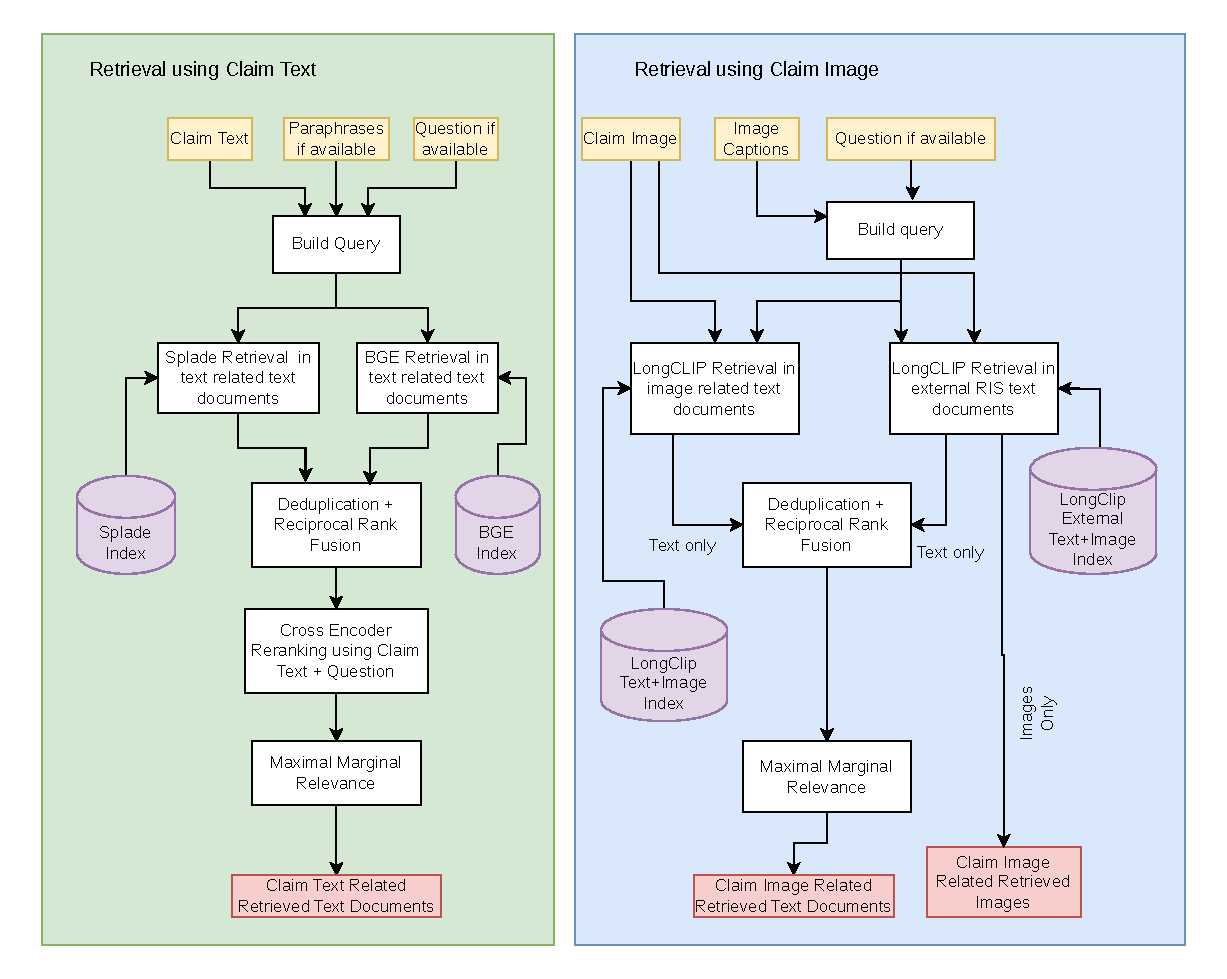
\includegraphics[width=\textwidth]{images/NewNewRag.pdf}
\caption{Hybrid Multimodal Dual-Branch Retriever (Dual-RAG). The yellow sections are the inputs and red sections are the outputs of RAG. The purple sections are the different indexes for the specific retrieval methods}
\label{fig:rag}
\end{figure}

In this thesis, we refer to our \textit{Hybrid Multimodal Dual-Branch Retriever} as \textit{Dual-RAG}. Dual-RAG separates evidence retrieval into text-based and image-based branches. The objective of this separation is to preserve strong lexical and semantic signals from claim text while also capturing cross-modal visual evidence from claim images.

\subsubsection{Text-Based Retrieval Branch}

The text-based branch retrieves evidence from textual knowledge store documents using two complementary retrievers:
\begin{itemize}
    \item \textbf{BGE} for dense semantic similarity,
    \item \textbf{SPLADE} for sparse lexical matching.
\end{itemize}

Retriever-specific queries are constructed from the claim text, its paraphrases and the fact-checking question when available. This branch is designed to capture both semantic paraphrases and exact lexical details (entities, dates, numbers, and quoted claims).

\subsubsection{Image-Based Retrieval Branch}

The image-based branch retrieves evidence using LongCLIP with multimodal inputs derived from claim images and their captions, together with the verification question when available. This branch searches both image-related textual and visual spaces to retrieve:
\begin{itemize}
    \item text passages aligned with the visual content,
    \item related images from the knowledge store.
\end{itemize}

By isolating this branch from the text-only branch, the system avoids over-dominance of textual signals and improves retrieval of visually grounded evidence.

\subsection{Reciprocal Rank Fusion (RRF)}

Different retrieval methods produce scores on incompatible scales, causing some modalities to dominate during fusion. Reciprocal Rank Fusion (RRF) avoids this issue by combining results based on rank positions rather than raw scores, providing more balanced and robust multimodal retrieval across heterogeneous data sources while remaining computationally efficient and parameter-light ~\cite{RyanBogan2025Nov}.

RRF assigns a score to every document based on its rank in each retrieval list using the formula:

\begin{equation}
    \text{RRF\_score}(d) = \sum_{r \in R} \frac{1}{k + \text{rank}_r(d)}
\end{equation}
where $k$ is a constant (commonly set to 60) that controls the influence of lower-ranked documents, $R$ is the set of retrieval lists, and $\text{rank}_r(d)$ is the rank of document $d$ in retrieval list $r$.

This allows documents from different sources or search queries with different distributions and retrieval characteristics to be compared on a consistent scale. In the text-based branch, RRF fuses BGE and SPLADE ranked outputs. In the image-based branch, RRF is not used, as it has a single retreival source as LongCLIP. RRF passes the top 50 documents to the deduplication stage.

\subsection{Deduplication}

Deduplication reduces redundancy in retrieved evidence, ensuring diverse and non-repetitive content for downstream reasoning. Duplicates based on url are not removed as, the different chunks providing different information could be retrieved for the same url. However near-duplicates are filtered using Jaccard similarity over token sets, discarding candidates with similarity above a threshold ($\tau$=0.85). This strategy preserves semantically distinct evidence while eliminating repetitive passages, improving evidence diversity and coverage.

The Jaccard similarity between two sets $A$ and $B$ is defined as:
\[
J(A, B) = \frac{|A \cap B|}{|A \cup B|}
\]

where $|A \cap B|$ is the size of the intersection of the two sets, and $|A \cup B|$ is the size of their union. This metric is used to measure the similarity between two sets of tokens, ensuring that near-duplicate content is filtered out.

\subsection{Cross-Encoder Reranking}

Although Reciprocal Rank Fusion (RRF) effectively combines results from multiple retrieval systems, it relies solely on ranking positions and does not explicitly model the semantic relationship between a claim and a retrieved document. To refine the retrieved evidence, a cross-encoder reranking stage is applied after RRF.

This work employs the \texttt{BAAI/bge-reranker} model as a second-stage reranker. Given a claim $q$ and a retrieved document $d$, the cross-encoder jointly processes both texts and produces a relevance score:

\begin{equation}
r(q,d) = f_{\text{CE}}(q,d)
\label{eq}
\end{equation}

where $f_{\text{CE}}$ denotes the cross-encoder and $r(q,d)$ is the predicted relevance score.

Unlike bi-encoder retrieval models, which encode queries and documents independently, the cross-encoder processes the claim and document simultaneously using the input format:

\begin{center}
\texttt{[CLS] claim [SEP] document [SEP]}
\end{center}

This allows the transformer to apply full self-attention across both texts and capture fine-grained interactions between claim and evidence tokens. The documents returned by RRF are reranked according to their cross-encoder scores, and the top-ranked 20 documents are forwarded to the subsequent Maximal Marginal Relevance (MMR) stage for diversification.

This enables the model to capture fine-grained interactions between claim and evidence tokens, including entities, contextual relationships, and factual statements. As a result, the reranker can distinguish between documents that are merely semantically related and those that provide evidence directly relevant to the claim.

Cross-encoders provide a favorable trade-off between retrieval quality and computational cost. Although they are more expensive than first-stage retrievers such as SPLADE and BGE, they are significantly more efficient than using Large Language Models (LLMs) for document reranking while still providing strong relevance estimation capabilities ~\cite{Dejean2024Mar}.

In the proposed pipeline, cross-encoder reranking is applied only to the textual retrieval branch after Reciprocal Rank Fusion (RRF). The image retrieval branch is not reranked because the selected BGE reranker is a text-only model and reranks the documents here based on the claim text which is not suitable to rerank documents retrieved based on the claim image. Instead, image-related evidence retrieved by LongCLIP proceeds directly to the subsequent diversification stages.

\subsection{Maximum Marginal Relevance (MMR)}

After cross-encoder reranking, the top-ranked documents are further processed using Maximum Marginal Relevance (MMR) to increase evidence diversity. News articles frequently contain duplicated reports, syndicated content, and highly similar passages. Without diversification, the final evidence set may contain multiple documents conveying essentially the same information.

MMR balances document relevance against redundancy by iteratively selecting documents that are both relevant to the query and dissimilar to previously selected documents. The selection criterion is defined as

\begin{equation}
\operatorname{MMR}
=
\arg\max_{d_i \in D \setminus S}
\left[
\lambda \cdot \operatorname{Sim}(d_i,q)
-
(1-\lambda)
\cdot
\max_{d_j \in S}
\operatorname{Sim}(d_i,d_j)
\right]
\label{eq:mmr}
\end{equation}

where $D$ denotes the set of candidate documents, $S$ denotes the set of previously selected documents, $q$ is the query, $\operatorname{Sim}(d_i,q)$ measures query-document relevance, $\operatorname{Sim}(d_i,d_j)$ measures document-document similarity, and  $\lambda \in [0,1]$ controls the trade-off between relevance and diversity. A value of $\lambda=1$ ranks documents solely based on query relevance, while $\lambda=0$ prioritizes diversity without considering relevance.

In the proposed pipeline, $\lambda=0.5$ was selected to give equal importance to relevance and diversity. This encourages the retrieval of complementary evidence while reducing redundancy among the selected documents. After diversification, the top 10 documents are forwarded to the question-answer generation stage.

The complete retrieval pipeline, consisting of SPLADE, BGE, LongCLIP, Reciprocal Rank Fusion (RRF), Deduplication, Cross-Encoder reranking, and MMR diversification, is referred to as \textit{Dual-RAG Evidence Retrieval} throughout the remainder of this thesis.



\section {Iterative Question-Answer Generation}
\label{section:iterative}

\begin{figure}[ht]
\centering
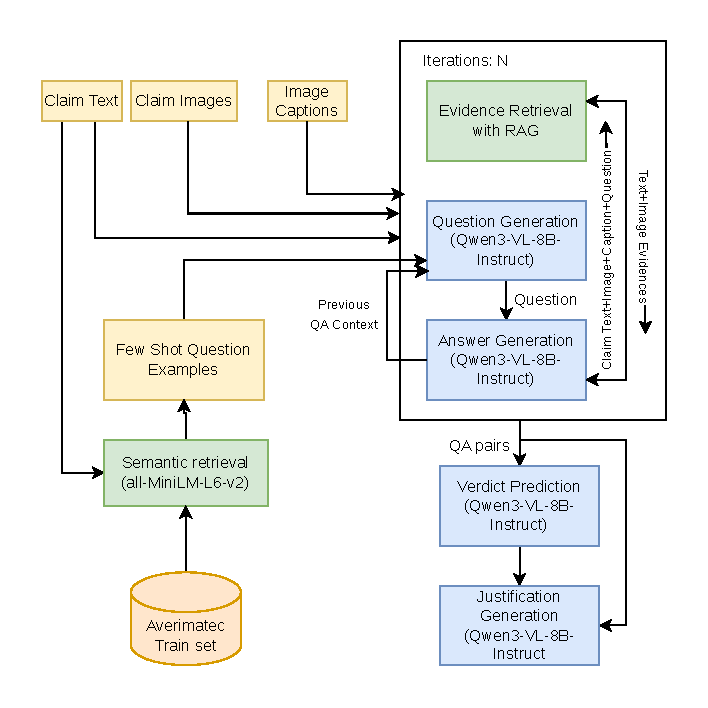
\includegraphics[width=\textwidth]{images/IterativeQA.pdf}
\caption{Iterative Question-Answer generation. The green sections are the retrieval methods, blue sections are for VLM based reasoning and generation, and yellow sections are the inputs to the VLMs}
\label{fig:iterativeEvidenceRetrieval}
\end{figure}

The iterative question-answer generation pipeline, illustrated in Figure~\ref{fig:iterativeEvidenceRetrieval}, performs fact verification through repeated cycles of question generation, evidence retrieval, and answer generation. The generated answers are incorporated into the context for subsequent iterations, allowing the system to accumulate evidence before producing a final verdict and justification.

\subsection{Question Generation}

The question generation module receives the claim text, claim images, and any previously generated question-answer pairs as input. A Vision-Language Model (VLM) generates verification questions that are subsequently used to retrieve evidence from the multimodal knowledge store.

The iterative pipeline performs two retrieval-reasoning iterations. During each iteration, the VLM generates three verification questions consisting of two text-related questions and one image-related question. After evidence retrieval, answers are generated and appended to the accumulated context. The question-answer pairs generated during the first iteration are provided as input when generating questions for the second iteration, enabling the model to avoid redundant questions and focus on unresolved aspects of the claim. Consequently, a maximum of six question-answer pairs are generated for each claim.

\subsubsection{Question Types}

The system generates two categories of verification questions:

\begin{itemize}
    \item \textbf{Text-related questions:} These target factual assertions in the claim text, such as dates, events, locations, names, and statistics. They are answered using textual evidence retrieved from the knowledge store. For example, given a claim about ``a 101-year-old woman giving birth,'' a text-related question might be: ``What is the maximum documented age for natural childbirth?''
    \item \textbf{Image-related questions:} These target the visual content of the claim image, addressing what is depicted, whether the image has been reused or manipulated, and whether it matches the textual narrative. Each image-related question includes an image index specifying which claim image it refers to. For example: ``What is the original source and context of this photograph [IMG\_1]?''
\end{itemize}

Question categorization determines which retrieval branch is used during evidence retrieval. Text-related questions utilize the textual retrieval pipeline, while image-related questions utilize the image retrieval pipeline.

\subsubsection{In-Context Learning for Question Generation}
\label{subsection:icl}

To guide question generation, the system retrieves the five most semantically similar training claims and uses them as in-context learning (ICL) demonstrations. Similarity is computed using sentence embeddings generated by the \texttt{all-MiniLM-L6-v2} model and cosine similarity:

\begin{equation}
\text{sim}(c,c_j)
=
\frac{\mathbf{e}_c \cdot \mathbf{e}_{c_j}}
{\|\mathbf{e}_c\| \, \|\mathbf{e}_{c_j}\|}
\label{eq:icl_cosine_similarity}
\end{equation}

where $c$ denotes the input claim, $c_j$ denotes the $j$-th training claim, and $\mathbf{e}_c$ and $\mathbf{e}_{c_j}$ are their corresponding sentence embeddings.

The top five most similar claims are selected as demonstrations:
\begin{equation}
\mathcal{D}_{\text{ICL}}
=
\operatorname{TopK}_{j}
\left(
\text{sim}(c,c_j),\, k=5
\right)
\label{eq:icl_topk}
\end{equation}

where $\mathcal{D}_{\text{ICL}}$ denotes the set of retrieved demonstrations.

For each selected example, the associated verification questions are extracted and included in the prompt. These demonstrations provide examples of the expected question style, structure, and level of detail, enabling the VLM to generate more targeted verification questions for the input claim.


The formatted examples are assembled into a structured ICL block:

\begin{verbatim}
Example Claim text 1: [similar claim text]
Example Questions:
**Text-related:** What is the origin of this event?
**Image-related:** Who is depicted in this photograph? **Image Index:** 1.

Example Claim text 2: [another similar claim]
...
\end{verbatim}

These examples demonstrate the expected question format, depth, and diversity to the generation model without prescribing the exact content of the questions for the current claim.

\subsubsection{Prompt Construction}

Question generation is formulated as a prompting task for the VLM. The prompt consists of three components:

\begin{enumerate}
\item A system instruction defining the task, output format, and generation constraints.
\item Optional in-context learning demonstrations retrieved using the procedure described above.
\item The target claim, associated images, and previously generated question-answer pairs from earlier iterations.
\end{enumerate}

The VLM is instructed to generate two text-related questions and one image-related question at each iteration while avoiding duplication with previously generated questions. Question generation is performed with a temperature of 0.5 to encourage diversity while maintaining relevance to the claim. Complete prompt templates are provided in Appendix ~\ref{ch:appendix_question}.

\subsection{Evidence Retrieval and Answer Generation}

Once verification questions have been generated, each question is processed independently through an evidence retrieval and answer generation pipeline. The question is first passed to the Dual-RAG retrieval system described in Section~\ref{ch:rag}, which retrieves relevant textual and image-related evidence from the knowledge store based on the question type. The retrieved evidence is then used to generate an answer to the question. Finally, each question-answer pair is converted into a declarative evidence statement that is subsequently used for verdict prediction and justification generation.

\subsubsection{Image Captioning}
\label{subsection:caption}

Prior to retrieval, each claim image is processed using a Vision-Language Model (VLM) to generate a structured textual description. These descriptions provide a textual representation of the visual content and are used by the LongCLIP retrieval branch when matching claim images against image-related textual evidence stored in the knowledge store.

For each image, the VLM generates two fields:

\begin{itemize}
\item \textbf{Caption:} A concise factual description of the visible content.
\item \textbf{Context:} A short phrase summarizing the overall scene or event depicted in the image.
\end{itemize}

The captioning prompt is designed to prioritize retrieval-relevant information, including named entities, visible text, objects, locations, and distinctive visual characteristics. The model is instructed to describe only directly observable content and to avoid speculation beyond the information present in the image.

The generated captions and context descriptions are subsequently used during LongCLIP retrieval to improve alignment between visual claims and image-related textual evidence.

\subsubsection{Answer Generation}

Given a verification question and the retrieved evidence, the answer generation module produces an evidence-grounded answer using the same Vision-Language Model (VLM) employed throughout the pipeline. The module receives the claim text, verification question, retrieved evidence documents, and any available claim metadata as input.

The retrieved evidence consists of the top-ranked documents returned by the Dual-RAG retrieval pipeline. When available, claim metadata such as the publication date and geographical location are also provided to supply additional temporal and contextual information that may assist in resolving ambiguous claims.

For image-related questions, references to the relevant claim images are included in the prompt, allowing the VLM to jointly reason over the visual content and the retrieved evidence. The model is instructed to generate answers that are grounded exclusively in the supplied evidence and to avoid unsupported speculation.

Question answering is performed with a temperature of 0.5 to balance factual consistency and reasoning capability. The generated answer is subsequently paired with its corresponding verification question and forwarded to the evidence statement generation stage. Complete prompt templates are provided in Appendix~\ref{ch:appendix_answer}.

\subsection{QA-to-Evidence Conversion}
\label{qa_evidence_conversion}

After an answer is generated, the question-answer pair is converted into a declarative evidence statement using the same VLM with in-context learning. This conversion transforms interrogative question-answer pairs into assertive statements that are more suitable for downstream verdict prediction.

The conversion process preserves the factual content of the generated answer while reformulating it into a self-contained evidence statement. Image references are retained using image identifiers (e.g., \texttt{[IMG\_1]}) so that subsequent modules can explicitly reference the corresponding claim images during reasoning.

The resulting evidence statements are aggregated across all verification questions and combined with any retrieved image evidence to form the final evidence package supplied to the verdict prediction module. Complete prompt templates are provided in Appendix~\ref{ch:appendix_qa_conversion}.


\section{Claim Based Retrieval for QA pair generation}
\label{section:qa_gen_answering}

In addition to the iterative question generation strategy adopted by Team Factiverse, REVEAL and Xxp ~\cite{Tariq2026Mar}, this work also investigates a claim-based single-pass alternative to assess the trade-off between retrieval depth and error propagation similar to the ones employed by AIC-CTU and VILLAIN ~\cite{Ullrich2026Mar} ~\cite{Jung2026Mar}.

This approach introduces a \textit{Analysis Model} that performs evidence retrieval and QA generation in a single coordinated pass. This section describes the end-to-end pipeline as implemented in the final system, detailing how a multimodal claim is processed from input to a set of diagnostic question-answer pairs.

\begin{figure}[ht]
\centering
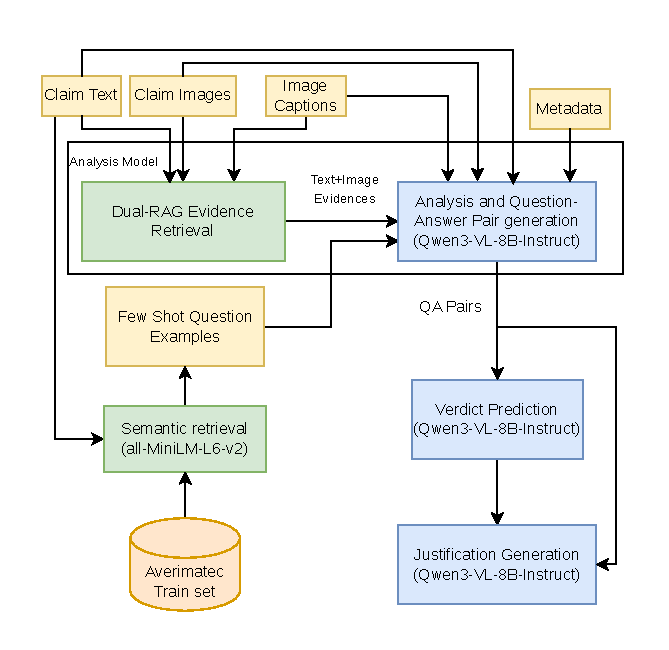
\includegraphics[width=\textwidth]{images/RetrievalQA.pdf}
\caption{Claim Based Retrieval for QA pair generation. The green sections are for the retrieval methods, blue sections are for VLM based reasoning and generation and yellow sections are the inputs to the VLM}
\label{fig:evidenceRetrievalFirst}
\end{figure}


\subsection{Pipeline Overview}

Given a multimodal claim consisting of textual content $c$, a set of associated images $\mathcal{I} = \{I_1, I_2, \ldots, I_m\}$, and metadata (date and location), the Analysis Model executes the following stages sequentially:

\begin{enumerate}
    \item \textbf{Image Captioning:} Generate textual descriptions of each claim image.
    \item \textbf{Query Augmentation:} Produce paraphrases of the claim text to expand retrieval coverage.
    \item \textbf{ICL Example Selection:} Retrieve semantically similar training examples for in-context learning.
    \item \textbf{Dual-Pass Evidence Retrieval:} Retrieve evidence through two complementary retrieval passes — text-only and image-augmented.
    \item \textbf{Prompt Construction:} Assemble the final prompt with claim, evidence, captions, metadata, and ICL examples.
    \item \textbf{QA Pair Generation:} Query the Vision-Language Model to produce structured diagnostic question-answer pairs.
\end{enumerate}

The complete pipeline is illustrated in Figure~\ref{fig:evidenceRetrievalFirst}.

\subsection{Image Captioning Stage}

The image captions are generated as described in section ~\ref{subsection:caption}. These captions serve a dual purpose: (1) they enable LongCLIP for text-text retrieval , and (2) they are included in the final QA generation prompt to provide the model with textual access to image information.

\subsection{Query Augmentation via Paraphrasing}

To improve retrieval recall, the system generates multiple paraphrases of the original claim text using the VLM.
 Paraphrasing serves to diversify the lexical and semantic representation of the claim, ensuring that retrieval captures evidence that may use different terminology to describe the same event or assertion. The paraphrases are concatenated with the original claim text to form an augmented query. This augmented query is used in subsequent retrieval passes to maximize coverage across different phrasings of the same factual assertions.

\subsection{In-Context Learning Example Selection}
Similar claim text and their corresponding questions are retrieved from the training examples to provide a guidance for Question generation as described in section \ref{subsection:icl}.


\subsection{Dual-Pass Evidence Retrieval}

A key design decision in the pipeline is the use of two separate retrieval passes that target complementary evidence signals. Rather than performing a single retrieval with all available information, the system executes:

\subsubsection{Pass 1: Text-Only Retrieval}

The first pass retrieves evidence using only the textual content of the claim and its paraphrases using the first retrieval pipeline defined by green section in Figure ~\ref{fig:rag}:

This pass focuses on identifying textual evidence that is semantically or lexically related to the claim's factual assertions, independent of any visual content. The retrieval passes through the Dual-RAG pipeline (BGE + SPLADE $\rightarrow$ RRF $\rightarrow$ cross-encoder reranking $\rightarrow$ MMR diversification), returning the top-10 most relevant text documents.

\subsubsection{Pass 2: Image-Augmented Retrieval}

The second pass incorporates the claim images and their captions using the second retrieval pipeline defined by blue section in Figure ~\ref{fig:rag}:

This pass activates LongCLIP's cross-modal retrieval capabilities, enabling the system to find evidence that is visually similar to the claim images or textually related to the image content and captions. This process returns the top 10 image related text documents along with 3 related images.

\subsubsection{Rationale for Dual-Pass Design}

The dual-pass strategy addresses a fundamental challenge in multimodal retrieval: image-augmented queries can sometimes overwhelm or dilute the textual signal, particularly when images are loosely related to the core factual assertion. By maintaining a separate text-only pass, the system ensures that purely textual evidence (e.g., fact-checking articles, news reports, official statements) is not lost in favor of visually similar but factually irrelevant content. Also sometimes the textual evidence from claim text dominate the textual evidence using the claim images and using a single text based cross encoder for the combined documents filtered using the claim text may dilute the textual documents retrieved using LongClip .The results from both passes are combined in the final evidence pool, providing the QA generation model with a diverse set of evidence spanning both text-grounded and image-grounded sources.

\subsection{Evidence Formatting}

The evidence documents from both retrieval passes are merged and formatted into a numbered list for inclusion in the prompt:

\begin{verbatim}
Document 1: [text from text-only retrieval]
Document 2: [text from text-only retrieval]
...
Document N: [text from image-augmented retrieval]
Document N+1: [text from image-augmented retrieval]
...
\end{verbatim}

Documents from the text-only pass appear first, followed by documents from the image-augmented pass. This ordering ensures that purely textual evidence is presented prominently, while image-related evidence provides supplementary context. The total number of documents presented to the model is bounded by the combined retrieval of top-20 from both passes.

\subsection{Prompt Assembly and QA Generation}

The final prompt is assembled by combining all processed inputs into a structured template that guides the VLM toward producing five diagnostic question-answer pairs. The prompt consists of claim text, claim images, captions, ICL examples, claim metadata and the retrieved evidences. It can be accessed in Appendix ~\ref{ch:appendix_analysis}.

The model generates a response with a temperature of 0.5, balancing factual grounding with sufficient diversity in the generated questions. The output is parsed as a JSON array, with validation ensuring that each element contains the required fields.

This single-pass architecture differs from the iterative approach described in earlier sections by generating all questions simultaneously with access to pre-retrieved evidence, rather than iteratively conditioning on previous answers. The trade-off is reduced computational cost (fewer VLM calls and retrieval operations) at the potential expense of adaptive question refinement. However, by providing the model with comprehensive evidence upfront, this approach enables the generation of more informed and evidence-grounded questions.

\section{Verdict Prediction and Justification Generation}

After Question-Answer Pair generation is completed for each of the approaches, the accumulated evidence is passed to two final modules: verdict prediction and justification generation. These modules operate sequentially — the predicted verdict is first determined from the evidence, and then a natural language justification is generated to explain the reasoning behind the verdict.

\subsection{Verdict Prediction}

The verdict prediction module determines the veracity of a claim using the evidence collected throughout the verification process. The module receives the claim text, claim images, available metadata, and the complete set of question-answer pairs as input and predicts a single verdict label using the same Vision-Language Model (VLM).

\subsubsection{Verdict Categories}

The system classifies each claim into exactly one of the following four verdict labels:

\begin{itemize}
    \item \textbf{Supported:} The evidence clearly supports the claim. This verdict is assigned when the retrieved evidence contains consistent and credible information that supports the factual assertions made in the claim.
    \item \textbf{Refuted:} The evidence contradicts the claim, or no credible support exists for it. This category is the preferred default when the system is uncertain — the prompt explicitly instructs the model to prefer ``Refuted'' over ``Not Enough Evidence'' in ambiguous cases. This design decision reflects the observation that claims submitted for fact-checking are more likely to be false than true.
    \item \textbf{Not Enough Evidence:} The retrieved evidence is completely irrelevant to the claim or insufficient to make any determination. This verdict is reserved for cases where the evidence simply does not address the factual assertions in the claim.
    \item \textbf{Conflicting:} The evidence is mixed or misleading that is some sources support the claim while others contradict it, or the evidence itself contains internally inconsistent information.
\end{itemize}

To ensure consistent outputs, the model is constrained to generate exactly one of the four predefined verdict categories. Inference is performed with a temperature of 0.2 to maximize determinism and reduce output variability. Complete prompt templates are provided in Appendix ~\ref{ch:appendix_verdict}

\subsection{Justification Generation}

After a verdict has been predicted, the justification generation module produces a textual explanation describing how the retrieved evidence supports the final decision. The module receives the claim text, claim images, claim metadata, aggregated question-answer pairs, and the predicted verdict as input.

Justification generation is performed using the same Vision-Language Model (VLM) employed throughout the pipeline. The model jointly reasons over the claim, evidence, and verdict to generate a coherent explanation that links the retrieved evidence to the predicted claim veracity.

This ordering with claim first, then evidence, then verdict is designed to encourage the model to reason about how the evidence connects to the claim before explaining the pre-determined verdict, rather than generating a post-hoc rationalization.

Inference is performed with a temperature of 0.2 to encourage focused and evidence-grounded explanations while maintaining consistency across claims. Complete prompt templates are provided in Appendix \ref{ch:appendix_justification}.

